\documentclass[tikz]{standalone}
\usepackage{amsmath}
\usetikzlibrary{positioning,3d,calc,angles}

\begin{document}

\begin{tikzpicture}

\node (obs) at (0, 0) {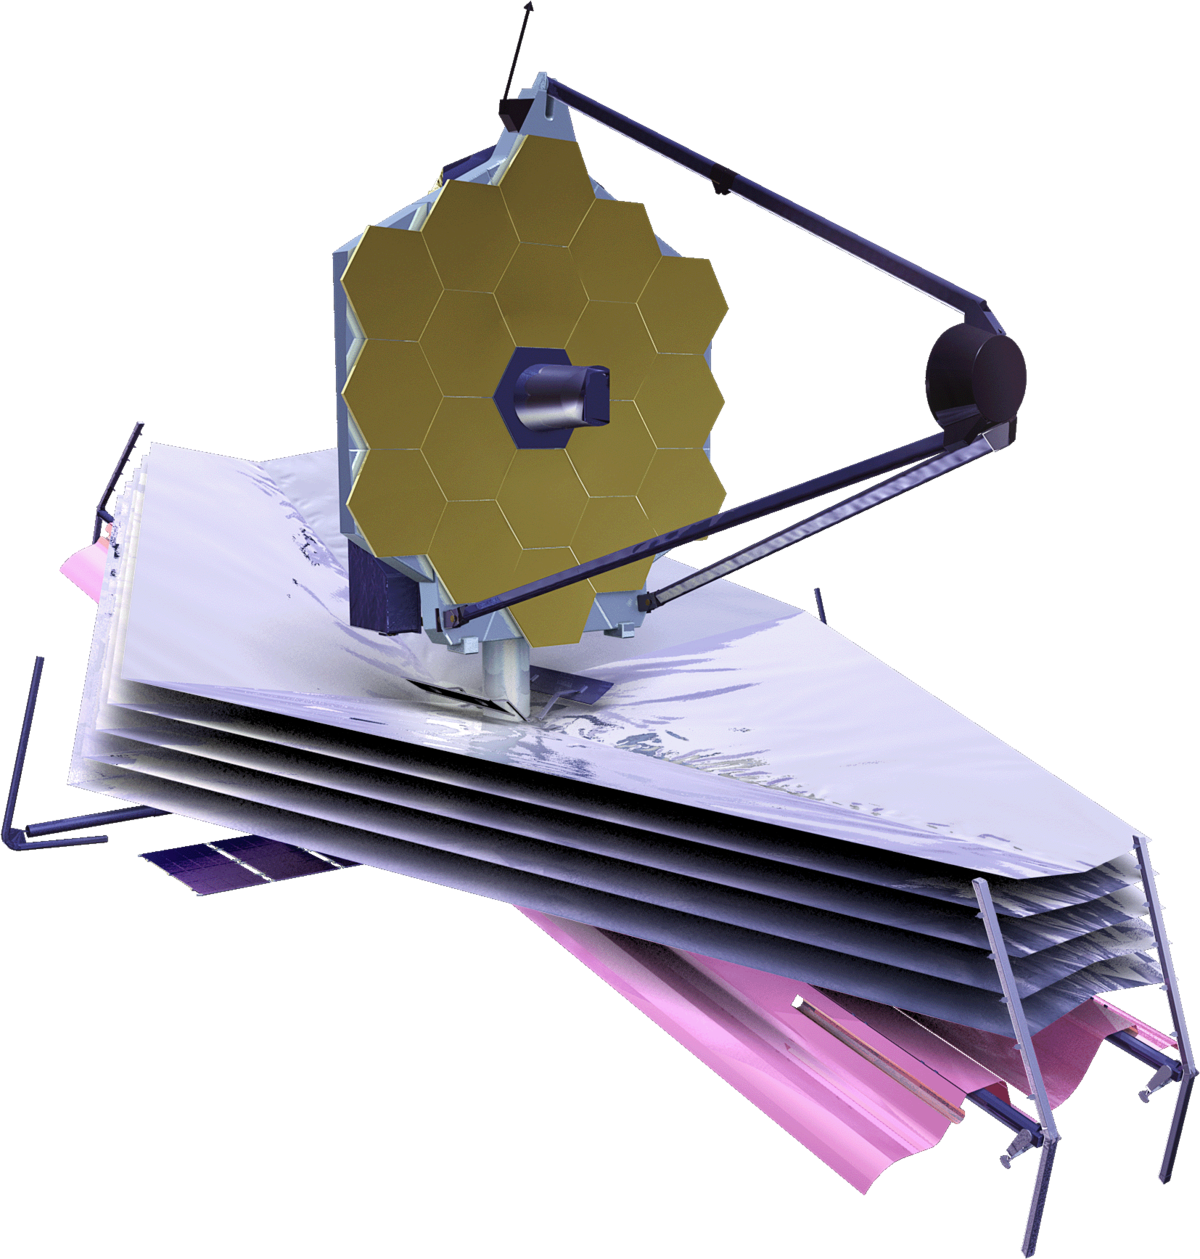
\includegraphics[width=2cm]{jwst_spacecraft}};

\draw (3, -1, -1) -- ++(0, 3, 0) -- ++(0, 0, 3) -- ++(0, -3, 0) -- ++(0, 0, -3); 
\draw (6, -1, -1) -- ++(0, 3, 0) -- ++(0, 0, 3) -- ++(0, -3, 0) -- ++(0, 0, -3); 

%rotate around y=45,rotate around z=30
\begin{scope}[canvas is zy plane at x=3, transform shape]
        \node (source) at (0.5, 0.5) {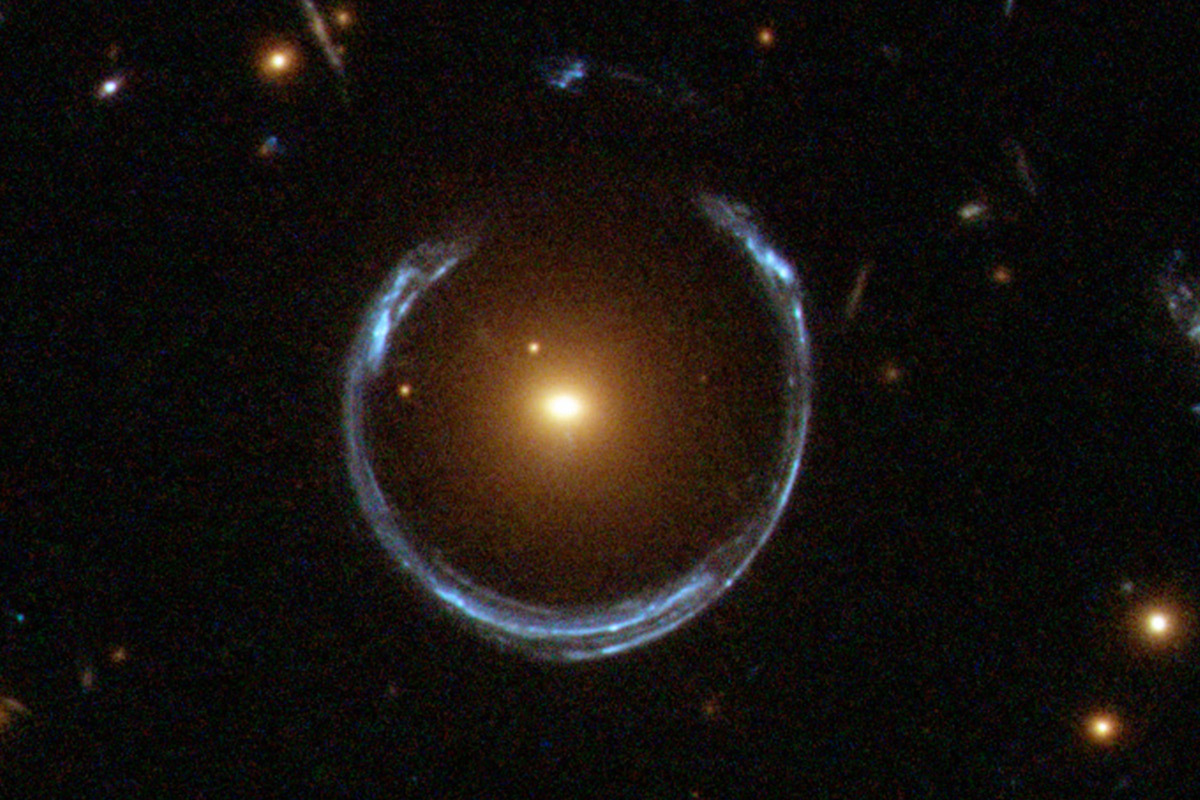
\includegraphics[width=3cm,height=3cm]{horseshoe_cropped.jpg}};
\end{scope}

\draw[latex-latex] (0, -1.9) -- (6, -1.9) node[midway, below] {$D_{s}$};
\draw[latex-latex] (0, -1.7) -- (3, -1.7) node[midway, above] {$D_{\ell}$};
\draw[latex-latex] (3, -1.7) -- (6, -1.7) node[midway, above] {$D_{\ell s}$};

\coordinate (s) at (0.56, 0.41) ;
\coordinate (p) at (0., 0.38) ;
\coordinate (h) at (-0.1, 0.6) ;
\draw[latex-] (p) -- (s) -- (h) -- +(3, 1) coordinate (theta0);
\draw[dashed] (theta0) -- +(3, 1);
\coordinate (xi0) at (3, 0.38);

\draw[dashed, color=black!70] (p) -- +(6, 0);

\draw (1, 0.96) .. controls +(0.25, -0.15) and +(0, 0.1) .. (1.2, 0.38) node[midway, right] {$\theta$};

\coordinate (s0) at (6, 0.5);
\draw (theta0) -- (s0); 

\draw (4, 1.95) .. controls +(0.2, -0.2) and +(0.1, 0.3) .. (4.2, 1.15) node[midway, right] {$\alpha$};

\draw[-latex, color=white] (3, -0.8, 1.5) -- +(0, 0, -0.5);
\draw[-latex, color=white] (3, -0.8, 1.5) -- +(0, 0.5, 0) node[near end, right] {$\boldsymbol{ \xi} $};

 
\end{tikzpicture}
\end{document}
